\documentclass{article}
\usepackage{arxiv}

\usepackage[utf8]{inputenc}
\usepackage[english, russian]{babel}
\usepackage[T1]{fontenc}
\usepackage{url}
\usepackage{booktabs}
\usepackage{amsfonts}
\usepackage{nicefrac}
\usepackage{microtype}
\usepackage{lipsum}
\usepackage{graphicx}
\usepackage{natbib}
\usepackage{doi}



\title{Распознавание почерка в рукописных документах}

\author{Кадченко Иван Евгеньевич \\
	ВМК МГУ\\
	\texttt{kadchenko.ivan@mail.ru} \\
	%% examples of more authors
	\And
	Местецкий Леонид Моисеевич \\
	ВМК МГУ\\
	\texttt{mestlm@mail.ru} \\
	%% \AND
	%% Coauthor \\
	%% Affiliation \\
	%% Address \\
	%% \texttt{email} \\
	%% \And
	%% Coauthor \\
	%% Affiliation \\
	%% Address \\
	%% \texttt{email} \\
	%% \And
	%% Coauthor \\
	%% Affiliation \\
	%% Address \\
	%% \texttt{email} \\
}
\date{2023}

\renewcommand{\shorttitle}{\textit{arXiv} Template}

%%% Add PDF metadata to help others organize their library
%%% Once the PDF is generated, you can check the metadata with
%%% $ pdfinfo template.pdf
\hypersetup{
pdftitle={Распознавание почерка в рукописных документах},
pdfsubject={q-bio.NC, q-bio.QM},
pdfauthor={Кадченко И.Е., Местецкий Л.М.},
pdfkeywords={First keyword, Second keyword, More},
}

\begin{document}
\maketitle

\begin{abstract}
	В данной работе предлагается метод распознавания почерка человека по его уникальному набору шаблонов. Пусть даны изображения рукописного текста и требуется определить, какое количество различных автором представлено на входных изображениях и к какому автору принадлежит каждый отдельный фрагмент текста. Решение данной задачи позволит устанавливать авторства различных документов, в том числе и исторических, а также упростить работу с архивами в целом. Предлагаемое решение опирается на штриховое представление рукописного текста. Гипотеза заключается в том, что каждый человек при написании различных букв использует примерно похожие, свойственнные ему движения руки, а также могут присутствовать какие-то штрихи, выделяющие конкретного автора.
\end{abstract}


\keywords{Распознавание почерка \and Шаблоны писателя \and Рукописные документы}

\section{Введение}
Распознавание почерка является одним из важнейших инструментов криминалистики, позволяющим идентифицировать автора документа или записи. Однако, существующие методы распознавания почерка требуют наличия текстовых образцов написания конкретного писателя, что затрудняет их применение в ряде случаев. В связи с этим, возникает необходимость в разработке методов распознавания почерка, которые не зависят от конкретного текста.

Один из таких методов - использование избыточных шаблонов, основанный на том, что каждый человек имеет свой индивидуальный почерк, который проявляется в определенных чертах написания букв и цифр. Эти черты могут быть выделены из большого числа образцов почерка и использованы для создания уникального шаблона писателя.

Актуальность проблемы независимого от текста распознавания почерка заключается в том, что это может помочь ускорить и улучшить процесс идентификации автора документов и записей. Например, при расследовании преступлений, где имеется только небольшой фрагмент написанного текста, использование избыточных шаблонов может значительно сократить время на поиск подходящих образцов почерка для сравнения. Кроме того, этот метод может быть полезен при работе с историческими документами или при анализе письменных свидетельств в судебных процессах. Таким образом, разработка методов независимого от текста распознавания почерка является актуальной и важной задачей для криминалистики и других областей, где требуется идентификация авторства документов и записей.

Данная работа будет направлена на поиск признаков для создания такого уникального шаблона писателя.

% \section{Headings: first level}
% \label{sec:headings}

% \lipsum[4] See Section \ref{sec:headings}.

% \subsection{Headings: second level}
% \lipsum[5]
% \begin{equation}
% 	\xi _{ij}(t)=P(x_{t}=i,x_{t+1}=j|y,v,w;\theta)= {\frac {\alpha _{i}(t)a^{w_t}_{ij}\beta _{j}(t+1)b^{v_{t+1}}_{j}(y_{t+1})}{\sum _{i=1}^{N} \sum _{j=1}^{N} \alpha _{i}(t)a^{w_t}_{ij}\beta _{j}(t+1)b^{v_{t+1}}_{j}(y_{t+1})}}
% \end{equation}

% \subsubsection{Headings: third level}
% \lipsum[6]

% \paragraph{Paragraph}
% \lipsum[7]



% \section{Examples of citations, figures, tables, references}
% \label{sec:others}

% \subsection{Citations}
% Citations use \verb+natbib+. The documentation may be found at
% \begin{center}
% 	\url{http://mirrors.ctan.org/macros/latex/contrib/natbib/natnotes.pdf}
% \end{center}

% Here is an example usage of the two main commands (\verb+citet+ and \verb+citep+): Some people thought a thing \citep{kour2014real, hadash2018estimate} but other people thought something else \citep{kour2014fast}. Many people have speculated that if we knew exactly why \citet{kour2014fast} thought this\dots

% \subsection{Figures}
% \lipsum[10]
% See Figure \ref{fig:fig1}. Here is how you add footnotes. \footnote{Sample of the first footnote.}
% \lipsum[11]

% \begin{figure}
% 	\centering
% 	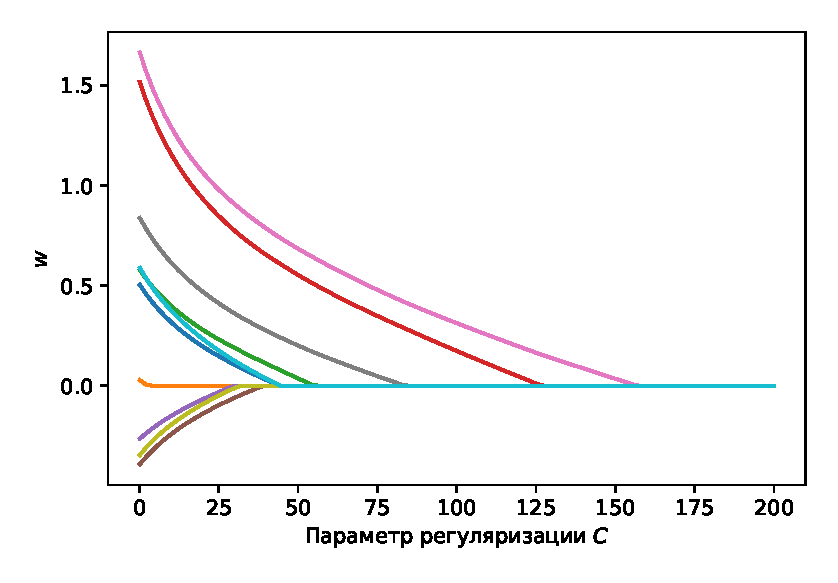
\includegraphics[width=0.5\textwidth]{../figures/log_reg_cs_exp.eps}
% 	\caption{Sample figure caption.}
% 	\label{fig:fig1}
% \end{figure}

% \subsection{Tables}
% See awesome Table~\ref{tab:table}.

% The documentation for \verb+booktabs+ (`Publication quality tables in LaTeX') is available from:
% \begin{center}
% 	\url{https://www.ctan.org/pkg/booktabs}
% \end{center}


% \begin{table}
% 	\caption{Sample table title}
% 	\centering
% 	\begin{tabular}{lll}
% 		\toprule
% 		\multicolumn{2}{c}{Part}                   \\
% 		\cmidrule(r){1-2}
% 		Name     & Description     & Size ($\mu$m) \\
% 		\midrule
% 		Dendrite & Input terminal  & $\sim$100     \\
% 		Axon     & Output terminal & $\sim$10      \\
% 		Soma     & Cell body       & up to $10^6$  \\
% 		\bottomrule
% 	\end{tabular}
% 	\label{tab:table}
% \end{table}

% \subsection{Lists}
% \begin{itemize}
% 	\item Lorem ipsum dolor sit amet
% 	\item consectetur adipiscing elit.
% 	\item Aliquam dignissim blandit est, in dictum tortor gravida eget. In ac rutrum magna.
% \end{itemize}


\bibliographystyle{unsrtnat}
\bibliography{references}

\end{document}
